\documentclass{article}
\usepackage{amsmath,amssymb,amsfonts,amsthm,fullpage,graphicx}

\newtheorem{problem}{Problem}

\begin{document}
\begin{flushright}
Kris Harper\\

CMSC 27500\\

April 8, 2009
\end{flushright}

\begin{center}
Homework 1
\end{center}

\begin{flushleft}

\begin{problem}
Show that:\\
1) Every path is bipartite.\\
2) A cycle is bipartite if and only if its length is even.
\end{problem}
\begin{proof}
1) Let $\{a_1, a_2, \dots , a_n\}$ be a path. Consider the two sets $V_1 = \{a_1, a_3, \dots\}$ and $V_2 = \{a_2, a_4, \dots\}$ of odd and even indices. Since every edge is of the form $(a_i, a_{i+1})$, there can be no edges which have both ends in one of these two sets. Thus every edge has one end in one set and one end in the other.\newline

2) Let $\{a_1, a_2, \dots , a_{n+1}\}$ be a cycle such that $a_{n+1} = a_1$ and $n$ even. Then the length of the cycle is even. As in Part 1), create two sets $V_1 = \{a_1, a_3, \dots , a_{n-1}\}$ and $V_2 = \{a_2, a_4, \dots , a_n\}$. From Part 1) we know the path from $a_1$ to $a_n$ is bipartite, so we only need to consider the edge connecting $a_n$ and $a_1$, which are in different sets. Thus, the cycle is bipartite. Conversely, suppose a cycle $\{a_1, a_2, \dots , a_{n+1}\}$ is bipartite. Let $V_1$ and $V_2$ be the two disjoint sets of vertices, and suppose that $a_1 \in V_1$. Then $a_2 \in V_2$. Inductively, if $a_i \in V_1$ then $a_{i+1} \in V_2$ where $i$ is odd. Since $a_n$ and $a_{n+1} = a_1$ must be in different vertex sets, it must be the case that $n$ is even.
\end{proof}

\begin{problem}
Let $G[X,Y]$ be a bipartite graph.\\
1) Show that $\sum_{v \in X} d(v) = \sum_{v \in Y} d(v)$.\\
2) Deduce that if $G$ is $k$-regular, with $k \geq 1$, then $|X| = |Y|$.
\end{problem}
\begin{proof}
1) If $d(v) = 0$ for all $v \in X$ then the problem is trivial. Let $v_1 \in X$ such that $d(v_1) \neq 0$. Then there exist edges $e_1 = (v_1, w_1), e_2 = (v_1, w_2), \dots e_n = (v_1, w_n)$. But note that since $G$ is bipartite, the vertices $w_1, \dots , w_n$ are in $Y$. Thus, for $v_1 \in X$ there are $d(v_1)$ vertices in $Y$ with degree at least $1$. Therefore $\sum_{v \in X} d(v) \leq \sum_{v \in Y} d(v)$. A similar result shows that $\sum_{v \in Y} d(v) \leq \sum_{v \in X} d(v)$. Therefore the two sums are equal.\newline

2) We have $k|X| = \sum_{v \in X} d(v) = \sum_{v \in Y} d(v) = k|Y|$. Since $k \geq 1$ we have $|X| = |Y|$.
\end{proof}

\begin{problem}
Let $G$ be a simple $k$-partite graph with parts of sizes $a_1, a_2, \dots , a_k$. Show that $m \leq \frac{1}{2} \sum_{i=1}^{k} a_i(n-a_i)$.
\end{problem}
\begin{proof}
Note that $(n-a_i)$ represents the number of vertices which are not in the $i$th part of the graph. Since no edge can have both ends in this part and the graph is simple, there can be at most $a_i(n-a_i)$ edges which have an end in the $i$th part. Summing over all $i$ parts gives us the total possible edges. But since every edge has two endpoints, only half of this number represents the total possible edges. Therefore, the number of edges in the graph must be less than or equal to $\frac{1}{2} \sum_{i=1}^{k} a_i(n-a_i)$.
\end{proof}

\begin{problem}
1) Show that $T_{k,n}$ has more edges than any other simple complete $k$-partite graph on $n$ vertices.\\
2) Determine $e(T_{k,n})$.
\end{problem}
\begin{proof}
1) Let $G$ be a complete $k$-partite graph on $n$ vertices with parts $A$ and $B$. Suppose that $|A| > |B| + 1$. That is, suppose that the difference in the two parts is greater than $1$. Now consider moving a vertex from $A$ to $B$. By doing this $G$ loses $B$ edges, but gains $|A| - 1$ edges. The total number of edges gained is then $|A| - 1 - |B|$, but we've assumed this is strictly greater than $0$. Thus the number of edges is maximized when the number of vertices in every part differs by no more than $1$. But this satisfies the conditions for the Tur\'{a}n graph.\newline

2) Using the formula from Problem 3 and substituting $n/k$ for $a_i$ gives the result
\[
m = \frac{n^2}{2} \left ( 1-\frac{1}{k} \right ).
\]
\end{proof}

\begin{problem}
1) Every eigenvalue of a graph is real.\\
2) Every rational eigenvalue of a graph is integral.
\end{problem}
\begin{proof}
1) Let $A$ the adjacency matrix of a graph. Note that $A$ is symmetric. Let $\lambda$ be a root of the characteristic polynomial of $A$. Then we have $Ax = \lambda x$ for some nonzero vector $x$. It's known that for two matrices, $M$ and $L$, we have $(ML)^T = L^T M^T$. Thus, we have $x^T A = \lambda x^T$. Note that $A^T = A$ and $\overline{A} = A$. Then taking conjugates we have $\overline{x}^T A = \overline{\lambda} \overline{x}^T$. Therefore
\[
\overline{x}^T A x = \overline{x^T A} x = \overline{\lambda x^T} x = \overline{\lambda} \overline{x}^T x.
\]
Also,
\[
\overline{x}^T A x = \overline{x}^T \lambda x = \lambda \overline{x}^T x.
\]
Thus we have $\lambda \overline{x}^T x = \overline{\lambda} \overline{x}^T x$ and so $(\lambda - \overline{\lambda}) \overline{x}^T x = 0$. Since $x \neq 0$, $\overline{x}^T x \neq 0$. Therefore $\lambda = \overline{\lambda}$ and $\lambda \in \mathbb{R}$.\newline

2) Let $a_n \lambda^n + \dots + a_1 \lambda + a_0 = 0$ be the characteristic polynomial for an adjacency matrix $A$ where $\lambda = p/q$ and $(p,q) = 1$. Then it must be the case that $p \mid a_0$ and $q \mid a_n$. To see this substitute $\lambda = p/q$ and divide by $q^n$. Then we have
\[
0 = a_np^n + q(a_{n-1}p^{n-1}q^0 + \dots + a_0p^0q^{n-1}) = a_0q^n + p(a_np^{n-1}q^0 + \dots + a_1p^0q^{n-1}).
\]
Since all coefficients are integers and $(p,q) = 1$, we must have $q \mid a_n$. But note that for the adjacency matrix, the $a_n$ term is given by $(\lambda - b_{11})(\lambda - b_{22}) \dots (\lambda - b_{nn})$. Thus $a_n = \pm 1$. Therefore $q = \pm 1$ and $\lambda \in \mathbb{Z}$.
\end{proof}

\begin{problem}
Show that the following graphs are isomorphic:\\
\begin{center}
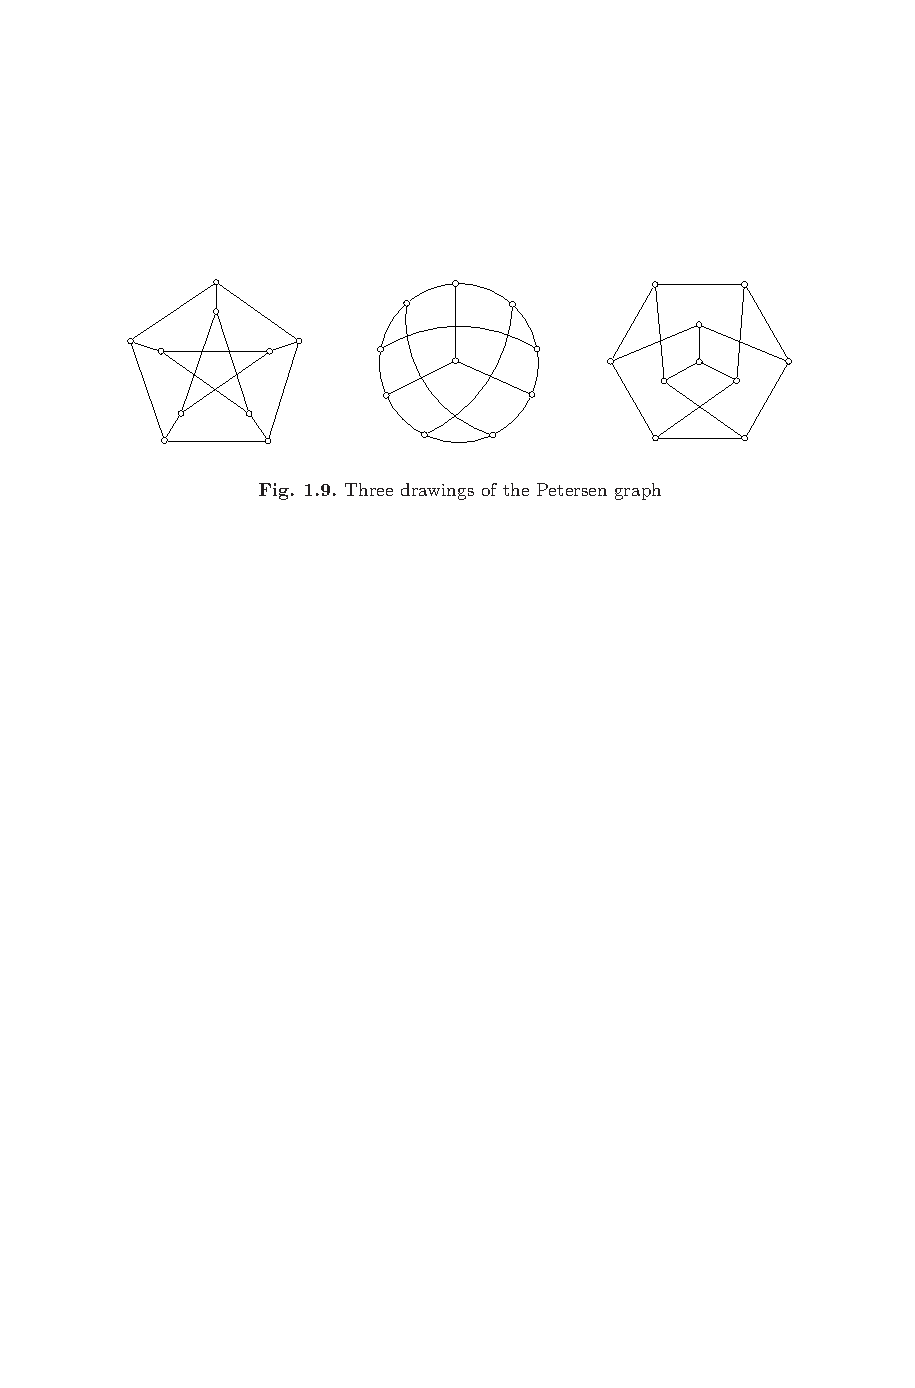
\includegraphics{Problem6}
\end{center}
\end{problem}
\begin{proof}
With the numberings as above, the following are isomorphisms between the first and second graphs, the second and third graphs and the third and fourth graphs respectively.
\[
\left (
\begin{array}{cccccccccc}
10 & 1 & 7 & 4 & 9 & 2 & 8 & 3 & 5 & 6\\
6 & 1 & 9 & 8 & 5 & 2 & 4 & 3 & 10 & 7
\end{array}
\right )
\]
\[
\left (
\begin{array}{cccccccccc}
10 & 7 & 9 & 8 & 6 & 3 & 1 & 4 & 5 & 2\\
10 & 1 & 7 & 4 & 9 & 2 & 8 & 6 & 5 & 3
\end{array}
\right )
\]
\[
\left (
\begin{array}{cccccccccc}
10 & 7 & 9 & 8 & 6 & 3 & 1 & 4 & 5 & 2\\
6 & 1 & 9 & 8 & 5 & 2 & 4 & 7 & 10 & 3
\end{array}
\right )
\]
\end{proof}

\end{flushleft}
\end{document}